\chapter{Improvements to basic algorithms}
\label{chap:imp}
In this chapter we improve algorithms presented in previous chapters and introduce a parallel method of testing pattern avoidance.

\section{General pattern}
We start by improving the brute force algorithm from Chapter \ref{chap:general}.

\subsection{Improving memory consumption}
The algorithm creates all possible partial mappings and checks whether at least one can be extended to a full mapping (mapping all lines of the pattern). To compute all the partial mappings of some level $l$, it only uses mappings of level $l-1$; therefore, it is enough to only store partial mappings of two levels in memory at any time.

In Chapter \ref{chap:general} we also introduced the notion of (un)important lines and equivalence based on not using unimportant lines at all (they are fully bounded by other already mapped lines). When a line becomes unimportant, it stays unimportant till the end of the test; as a result, we can forget where we mapped those lines to save memory and only remember where we mapped important lines.

\subsection{Not mapping empty lines}
\begin{defn}
An \emph{empty} line is a row or a column that does not contain any one-entries.
\end{defn}
An empty line can be mapped to any line and we do not need to map it at all, as long as the algorithm does not map two lines surrounding an empty one to two consecutive lines.

\subsection{Using the last changed position}
The MCMC process always changes one element of the big matrix and asks whether it still avoids the pattern. If it does not and we know that before the change it did, we are sure the changed element $[r,c]$ is a part of the pattern. It is hard to use this fact in the algorithm. It just maps one line after another and we do not know at the beginning to which line the changed position lines should be mapped.

What we can do is to enforce that neither the $r$-th line nor the $n+c$-th one ($c$-th column) get skipped. We only look at the restriction for rows as the restrictions for columns are symmetrical. There are three situations we want to avoid:
\begin{itemize}
\item The first row of $P$ is mapped under the $r$-th row. This prevents any other row to be mapped to $r$-th one and we do not want that.
\item The last row of $P$ is mapped above the $r$-th row. This again prevents any other row to be mapped to $r$-th one.
\item Two adjacent rows $l,l+1$ of $P$ are mapped to $L<L'$ respectively and $L<r<L'$ which leaves no other row to be mapped to $r$.
\end{itemize}

\subsection{Line order}
\label{sect:order}
An important thing, if we want the algorithm to run fast, is to choose a good line order. A line which is unimportant in level $l$ in a line order may easily be important till the nearly last level in a different order.

We choose line order to hopefully enforce two things:
\begin{itemize}
\item Make as many unimportant lines as possible. This really allows the equivalence based improvements to kick in. The more lines are unimportant the more mappings become equivalent and the faster it is to iterate through all of them.
\item Recognize hopeless partial mappings as soon as possible. A partial mapping gets extended if the line does not break the rule that there is a one-entry where it needs to be. If we map all the rows first, the rule will get broken only after we start to map columns and we probably want to find out sooner.\\
\end{itemize}
In the program a user can either choose their own custom order or one of five algorithms with different main purposes:
\begin{itemize}
\item AUTO - this one tries the other three line orders and chooses the one which shows the best performance over some iterations on a matrix. While this may sound like a good thing to use, it is only so if an initial matrix is chosen and it takes a lot of time since a lot of iterations need to be made in order to make a good sample. I would recommend not to use AUTO order at all and instead to try all the line orders by hand with a number of iterations depending on the pattern and a good initial matrix; for instance, generated with a smaller number of iterations on the same pattern and with any line order.
\item DESC - the lines are ordered in descending order depending on the number of one-entries. This follows the idea to start with the lines that are the hardest to map. Note that this algorithm does poorly if there are a lot of lines with the same number of one-entries (for example an identity matrix).
\item MAX - it orders the lines so that the maximum number of important lines throughout the levels is as small as possible. This focuses straightforwardly to having many unimportant lines, which the program does not remember.
\item SUM - it orders the lines so that the sum of the numbers of the important lines is the smallest possible throughout all levels. The purpose is the same as in the MAX order and quite often it is the case both approaches produce the same order.
\item TWO - it orders the lines so that the maximum number of important lines in two consecutive levels throughout all the levels is as small as possible. This again focuses to having many unimportant lines, which the program does not remember. The constant two is chosen due to the fact general pattern always stores two levels of partial mapping at a time.
\end{itemize}

\subsection{Mapping approaches}
\label{sect:approaches}
The one thing the approaches we will introduce have in common is that they try to recognize those partial mappings that have no chance to be extended to a full mapping as early as possible.

While the algorithm introduced in Chapter \ref{chap:general} finds out the partial mapping is invalid only at the time it maps two lines having a one-entry at their intersection to two lines having a zero-entry at the intersection, different approaches try to reveal the fact we would end up in the situation earlier by checking more conditions.
\begin{figure}[h!]
\centering
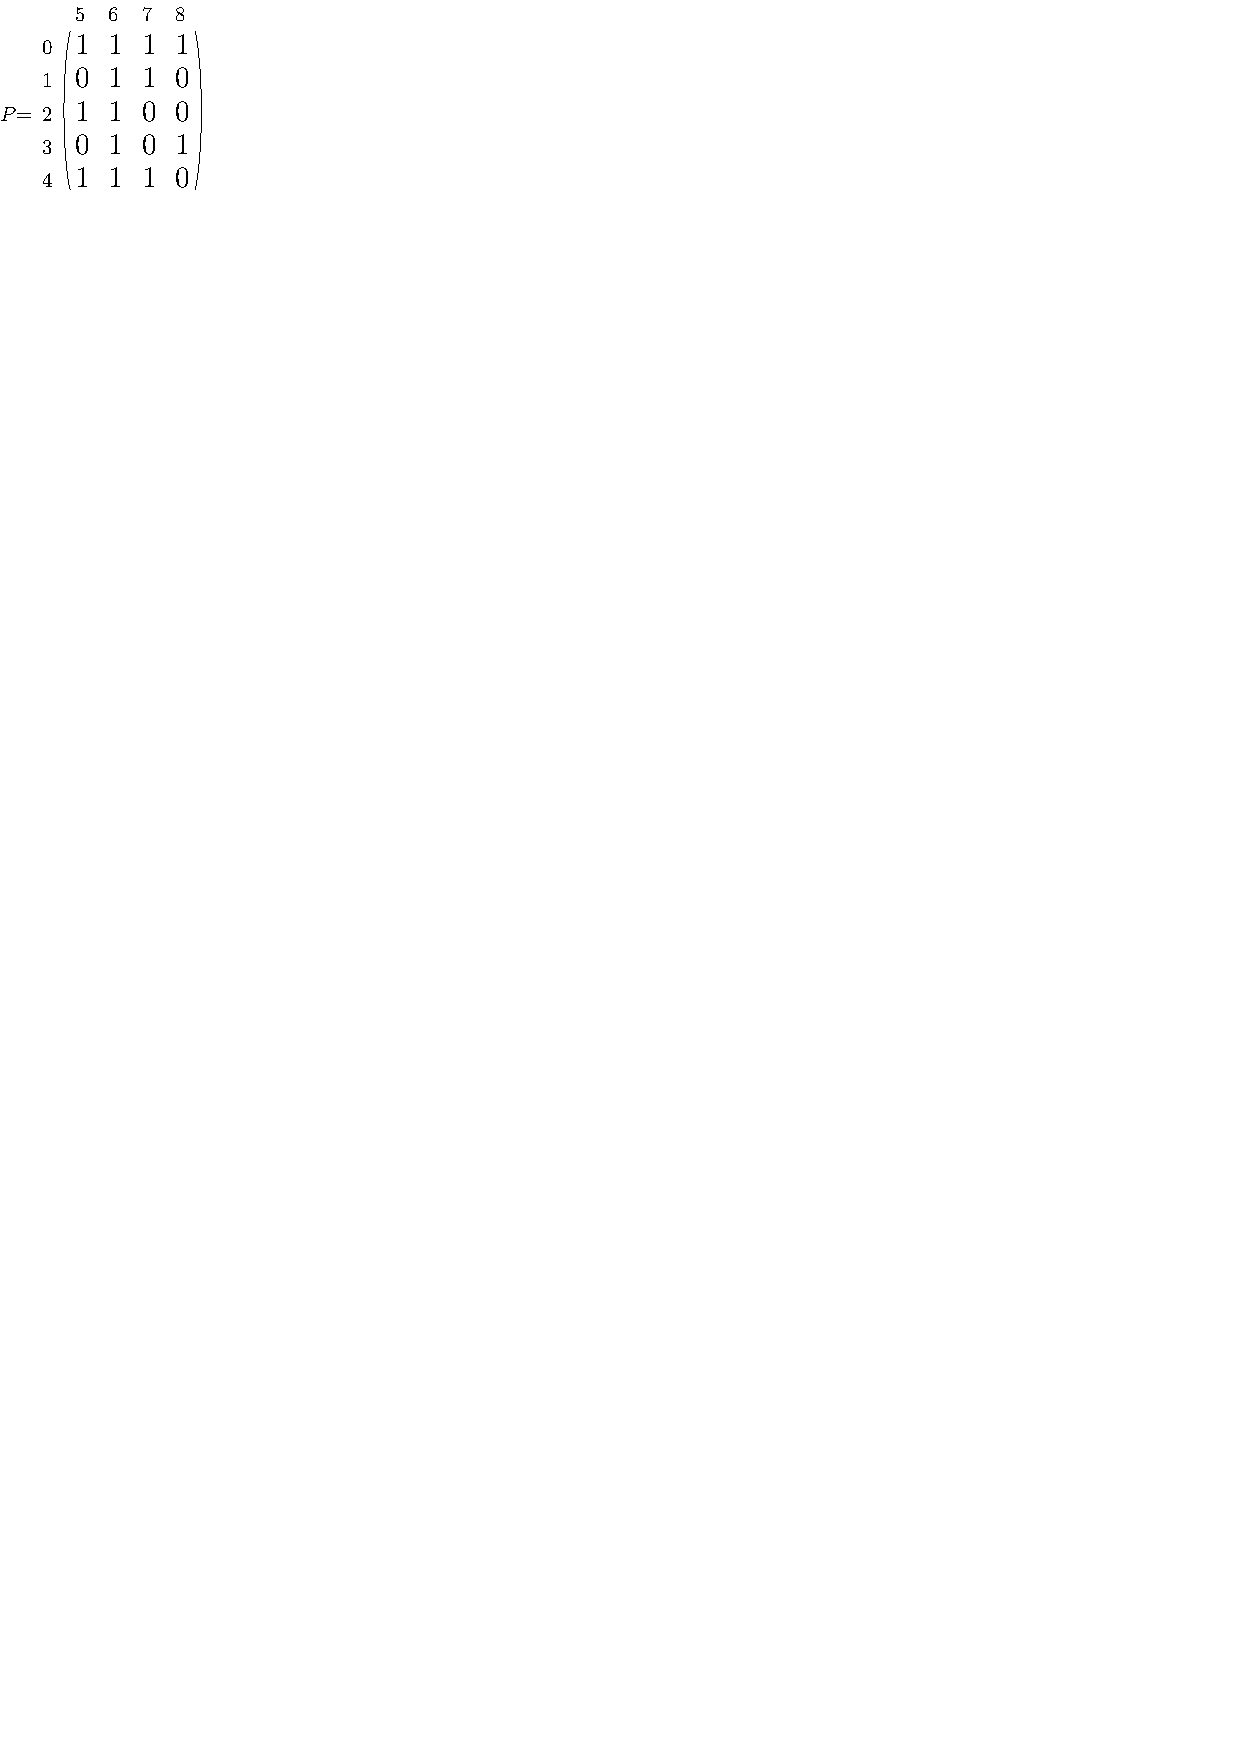
\includegraphics[width=60mm]{../img/approaches.pdf}
\caption{Pattern $P$ on which we demonstrate mapping approaches.}
\label{approaches}
\end{figure}
Let $P$ from Figure \ref{approaches} be the forbidden pattern and imagine a situation, in which only lines 0, 3 and 7 are mapped and line 6 is currently being mapped. There are a few necessary conditions we can check:
\subsubsection{Enough one-entries}
\begin{figure}[h!]
\centering
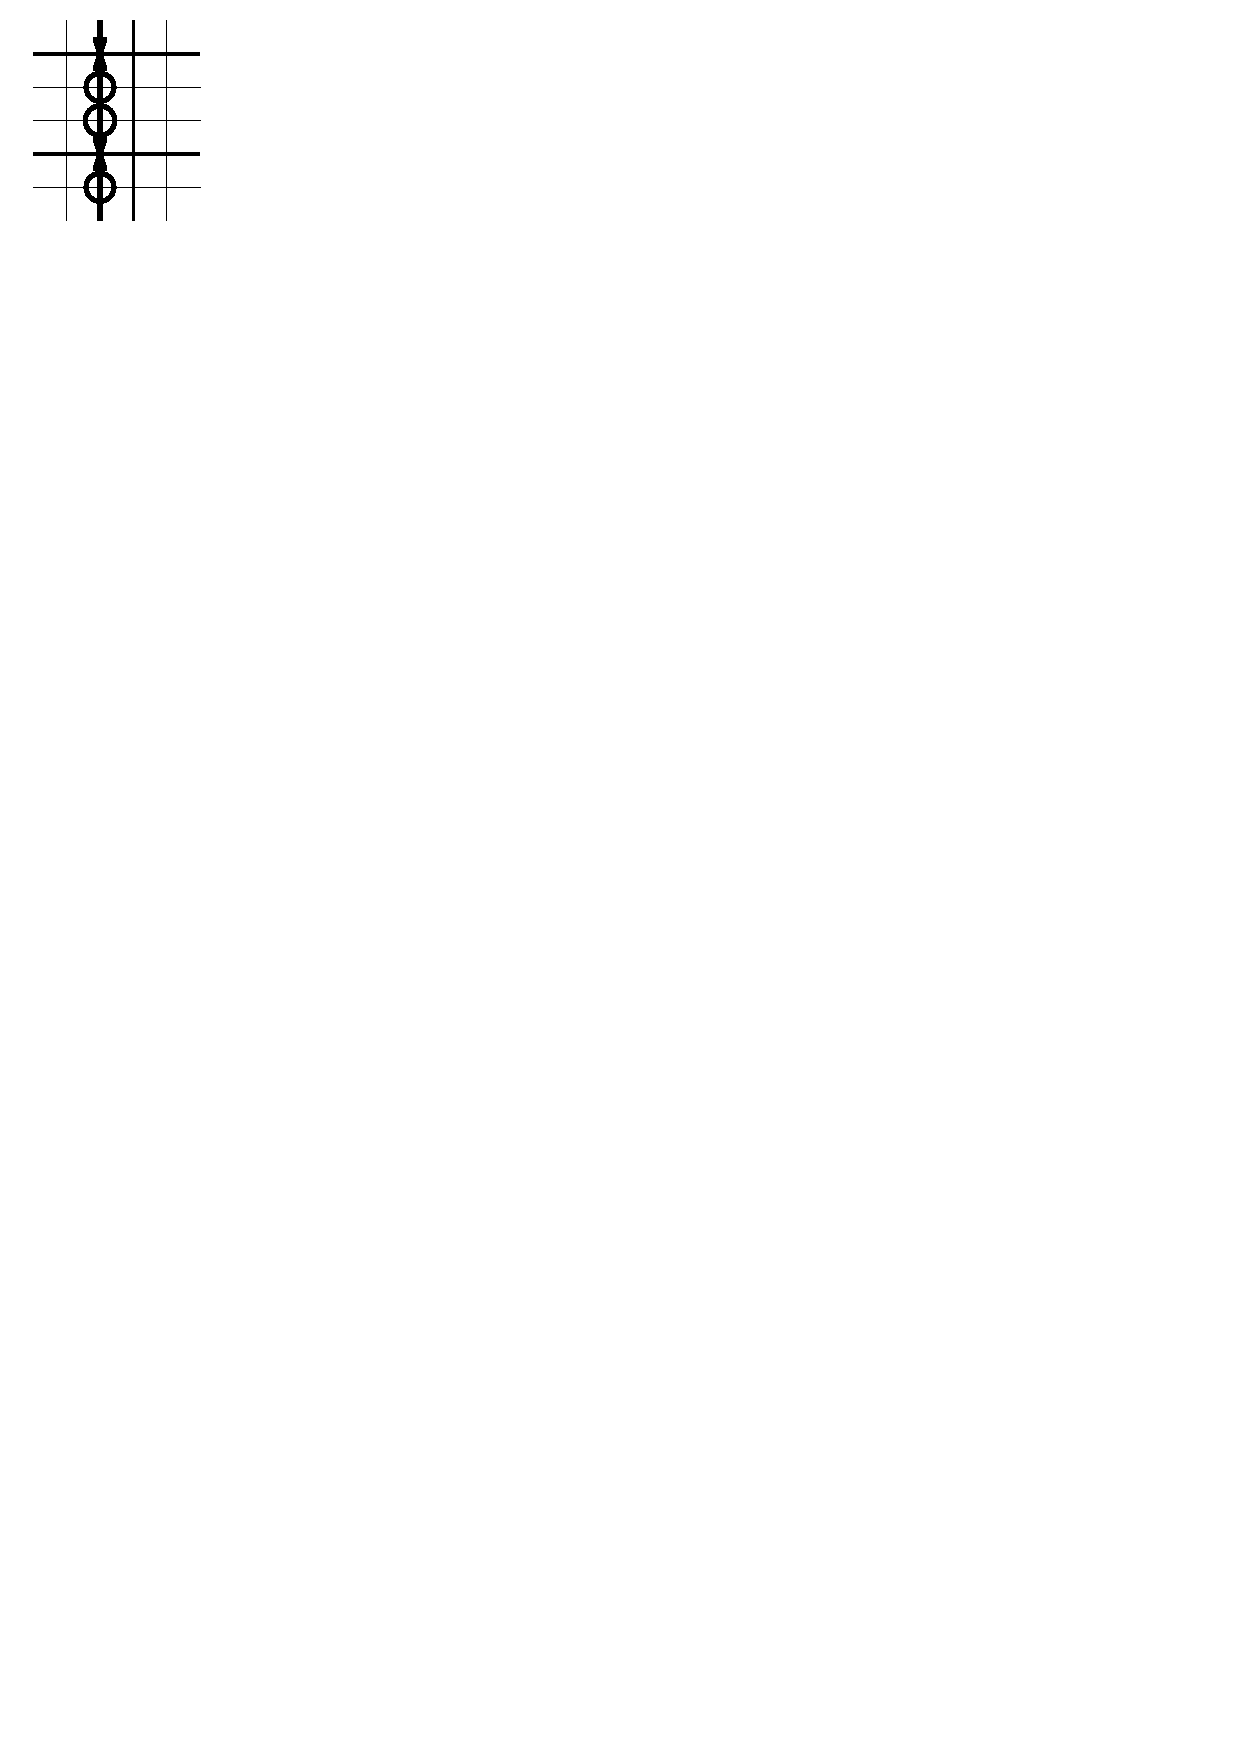
\includegraphics[width=55mm]{../img/enough_one-entries.pdf}
\caption{Checking whether there is enough one-entries. Bold lines in the picture are mapped and in circles are the positions where we look for one-entries.}
\label{enough}
\end{figure}
The first condition is that there is enough one-entries in between mapped lines, which is schematically shown in Figure \ref{enough}. We check whether there is enough one-entries on lines in between those lines, where lines 0 and 3 are mapped, so that there is a hope we can map lines 1 and 2 there. Similarly, we check whether there is a one-entry below the line, where line 3 is mapped so we can map line 4 there later.
\subsubsection{Recursive mapping}
\begin{figure}[h!]
\centering
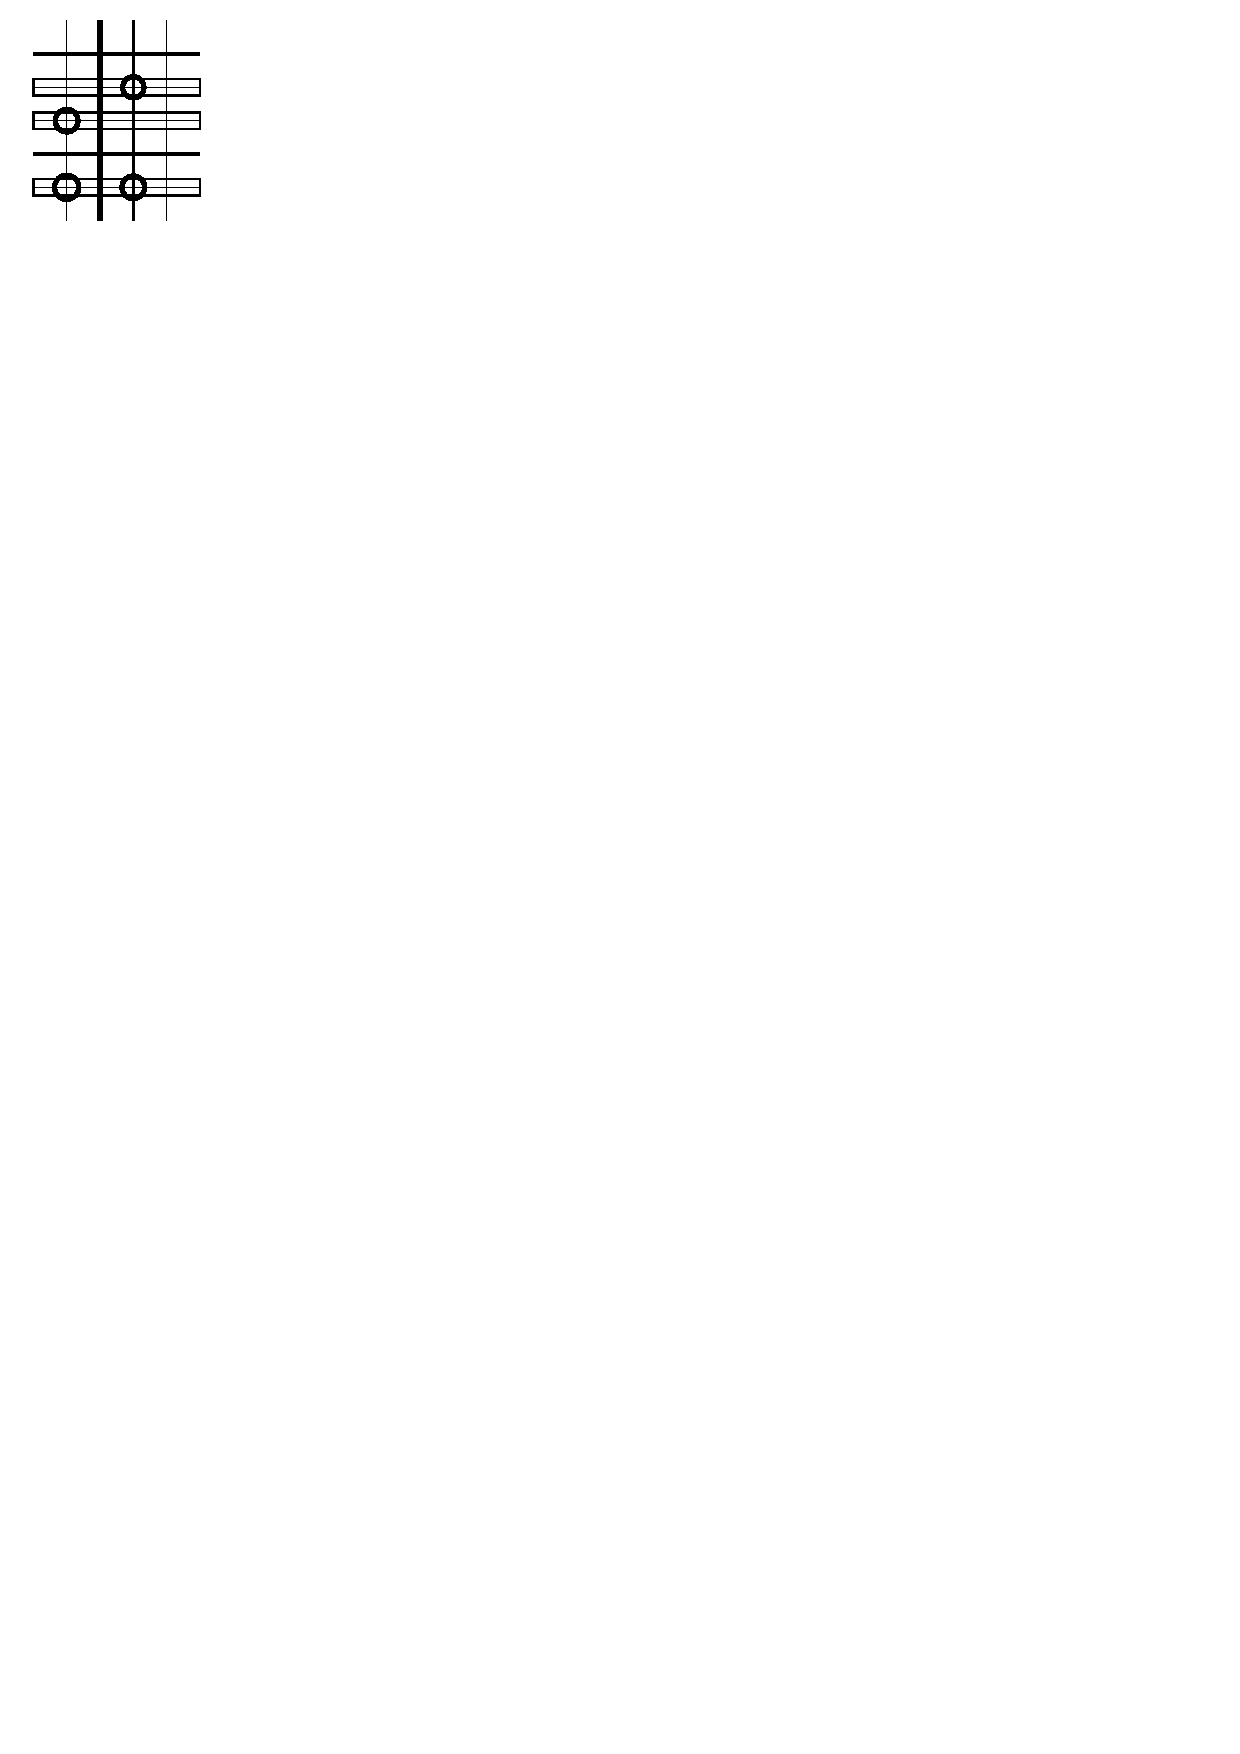
\includegraphics[width=55mm]{../img/recursive.pdf}
\caption{Checking whether crossed non-mapped lines can be mapped anywhere. Bold lines are mapped or being mapped, in rectangles are the lines we check and in circles are the positions where we look for one-entries.}
\label{recursive}
\end{figure}
While we were only testing whether there are enough one-entries in between already mapped lines in the previous approach, as you can see in Figure \ref{recursive}, this time we also check whether those one-entries can be used for the lines that are intended to be mapped there. For example, when we check there is a one-entry to be used for line 1 later, we also check the line 1 can be mapped to the row with one-entry, which in this situation means to also check there is a one-entry at the intersection with the line to which the line 7 is mapped.
\subsubsection{Orthogonal bounds}
\begin{figure}[h!]
\centering
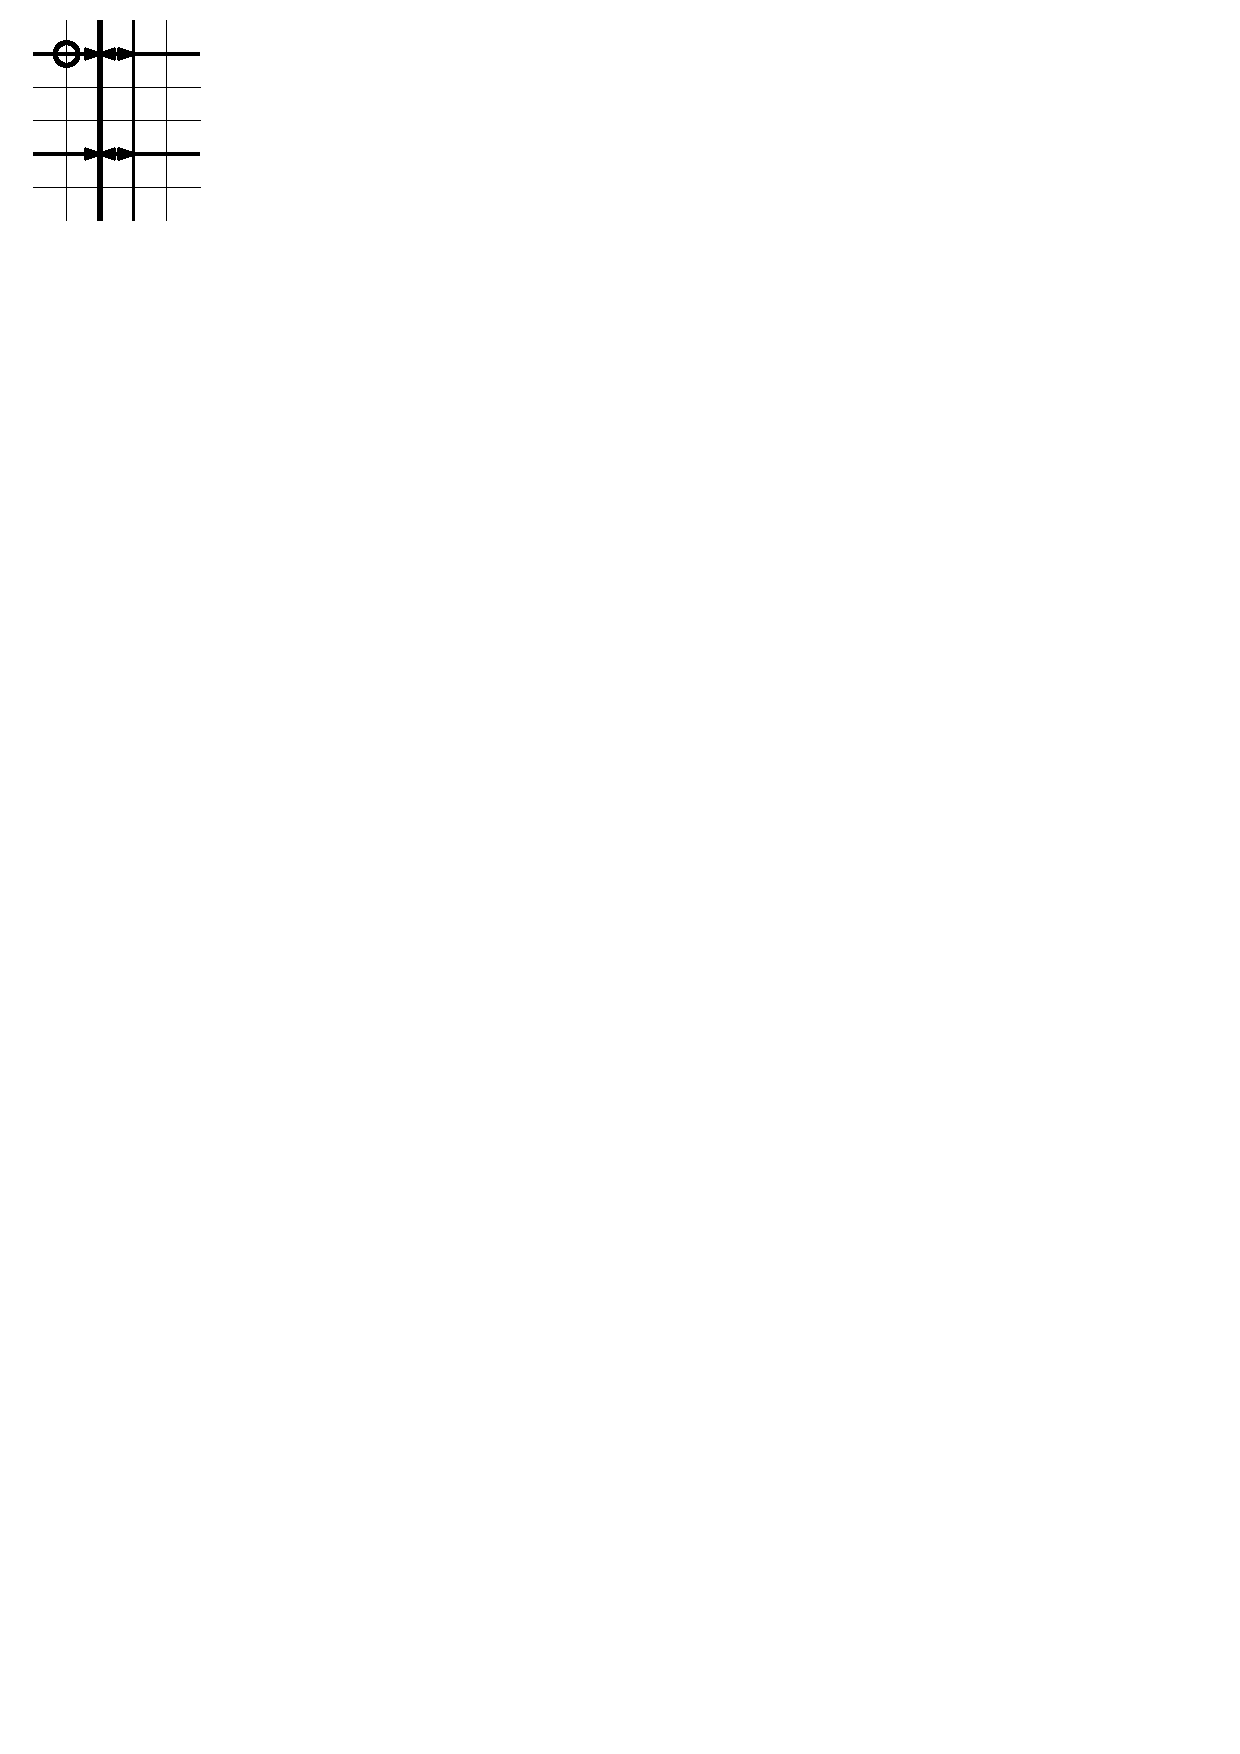
\includegraphics[width=55mm]{../img/orthogonal.pdf}
\caption{Checking whether there is enough one-entries on the orthogonal lines. Bold lines are mapped or being mapped and in circles are the positions where we look for one-entries.}
\label{orthogonal}
\end{figure}
As shown in Figure \ref{orthogonal}, when we are adding line 6, we check whether there is enough one-entries on the already mapped lines orthogonal to line 6 between line 6 and the closest mapped lines next to line 6. The idea is same as in ``Enough one-entries'', but we check different lines.

\subsubsection{Usage}
These restrictions on the added lines are not a fixed part of the program. A user can decide which approaches they want to use in the configuration file.

When testing that was done for a fixed pattern, we found out it is useful to use all the mentioned restrictions when generating a matrix avoiding some patterns while it was much better not to use any of those restrictions for different pattern, which you can see in Table \ref{approachestable}. For some patterns it also happened that using additional restrictions was useful for matrix of size $100\times100$ and for the same patterns it was better not to use them for generating a $500\times500$ matrix.
\begin{table}[]
\centering
\begin{tabular}{|ccc|c|r|c|c|c|r|r|}
\hline
\multicolumn{3}{|c|}{\textbf{Pattern}} & \textbf{n} & \textbf{\#iterations} & \textbf{one} & \textbf{rec} & \textbf{orth} & \textbf{time (sec)} & \textbf{memory} \\ \hline
1 & 0 & 0 & 100 & 100,000 & yes & yes & yes & 122.24 & 3,004 B \\ \cline{4-10} 
1 & 1 & 1 & 100 & 100,000 & no & no & no & 248.65 & 3,268 B \\ \cline{4-10} 
0 & 0 & 1 & 500 & 10,000 & yes & yes & yes & 1,072.53 & 5,380 B \\ \cline{4-10} 
  &   &   & 500 & 10,000 & no & no & no & 2,631.73 & 15,976 B \\ \hline
1 & 1 & 1 & 100 & 100,000 & yes & yes & yes & 1,512.56 & 3,268 B \\ \cline{4-10}
1 & 1 & 1 & 100 & 100,000 & no & no & no & 672.63 & 3,268 B \\ \cline{4-10} 
1 & 0 & 0 & 500 & 10,000 & yes & yes & yes & 10,276.60 & 9,128 B \\ \cline{4-10} 
  &   &   & 500 & 10,000 & no & no & no & 6,756.96 & 15,972 B \\ \hline
\end{tabular}
\caption{Testing additional restrictions of the generated matrix is useful in some cases but it comes with a performance drop in different cases.}
\label{approachestable}
\end{table}

\subsection{Using the whole structure in the next iteration}
\label{wholestructure}
It may seem like a good idea to store all the partial mappings. In the next iteration, instead of finding all the partial mapping again, we only alter the mappings we remember. Let $i$ be the number of the iteration we are in, and $e$ be the element.

If the element $e$ is changed from zero-entry to one-entry, for each partial mapping we have stored in previous iterations, we want to try to extend it only by the line that just changed. If we manage to extend a partial mapping, we then try to extend it to a full mapping in all possible ways (not only by using changed lines). When the new line in such a mapping becomes unimportant, we can stop looking for all possible extensions if the mapping is equivalent with a different one, which comes from previous iterations. This can be easily done by means already used in the standard algorithm.

However, if the element $e$ gets changed from one-entry to zero-entry we need to go through the partial mappings and delete all those that use $e$. This complicates the algorithm as we can no longer forget unimportant lines. Moreover, for each partial mapping we need to remember how many partial mappings of the previous level can be extended to that one, to delete that mapping from the list if there are no longer any mappings extensible to it.

This can all be done, but it comes with three huge inconveniences:
\begin{itemize}
\item Memory consumption - there can be a lot of partial mappings and we need to remember them all. We need to remember mappings of all levels and while we can still use the equivalence when extending a mapping, we need to also store all equivalent mappings for the purposes of deleting.
\item The change from one-entry to zero-entry is no longer for free. If this change is done, we already know the pattern is not contained in $M$, but we still need to do a lot of work to change the structure in order to use it in the next iteration.
\item Reverting - if the change is unsuccessful (the pattern is contained) we need to revert the change which means to completely revert all changes we did to the list of partial mappings. This can be either done by making a backup copy of the whole structure and override the structure if needed, which again is very costly as the structure is huge, or we can remember what partial mappings are new (or deleted) and we go through all partial mappings and remove (add) those. This means to iterate through the big structure one more time for every unsuccessful change.
\end{itemize}
After realizing these issues it no longer looks useful to me and this version of the algorithm is not a part of the implementation.

\section{MCMC parallelism}
\label{sect:parallel}
To speed up computations, it is often possible to use parallelism. In this section, we show how to make the MCMC generator parallel, while still allowing both types of the pattern.

While the serial MCMC generator in each iteration changes one element in the generated matrix and checks whether it still avoids forbidden patterns, the parallel version makes several iterations at once, one on each copy of the generated matrix. This means that while iteration $x$ is being computed by a thread, iteration $x+1$ can at the same time be computed by a different thread. The issue is that the iteration $x+1$ does not know what is going to be the state of the generated matrix at the time it should start. It expects iteration $x$ to fail - not change the generated matrix at all, counting on the fact, it is unlikely a change does not create a mapping of the pattern, and starts with the same matrix as iteration $x$. If iteration $x$ succeeds, then the computed iteration $x+1$ is invalid and the iteration is going to be recomputed again, starting with the correct matrix.

When the parallel version of MCMC generator is chosen and it is assigned $n$ threads, it creates $n-1$ private copies of the generated matrix and assigns one thread, called worker, to each of them. The last thread, which we call the main thread and which has exclusive access to the master copy of the generated matrix, makes one change of a bit in each private copy of the matrix and makes the corresponding worker check the avoidance.

The job of a worker is only to check if its copy of the matrix still avoids the pattern when one bit is changed. On the other hand, all synchronization is left to the main thread. As mentioned before, one iteration of the MCMC process can be recomputed several times. We still want the generator to satisfy the conditions we have for the Markov chain (more in Section \ref{sect:mmcmc}) in order to approximate a random matrix. To achieve that, if a computed iteration $x$ succeeds (and changes the generated matrix), all the other computed iterations that would follow after the iteration $x$ become invalid and they all have to be recomputed. The process ends when all iterations get computed.

For the sake of clarity, from now on, we will not be talking about iterations but about tasks. A task is basically one iteration of the MCMC process. The usefulness of this notation comes with an ID - a number, unique per task, assigned to each task, starting with 1 and always increasing. For a pair of consecutive iterations $x$ and $x+1$ it will always be the case that if task $a$ is the last task to compute iteration $x$ (which means the iteration does not get recomputed ever again after) and task $b$ is the last task to compute iteration $x+1$, then the ID of $a$ is lower then the ID of $b$. Also there is no point, in which two different tasks would be computing the same iteration at the same time. If tasks with IDs $a<b$ computed the same iteration, it must have been the case an earlier iteration succeeded when task with ID $a$ was computed and after it got removed, task with ID $b$ was assigned to recompute.

At any point in time, we only consider those tasks, that are being computed or those that wait to be processed (not those that have been processed), which means the lowest ID of tasks we consider increases in time.

When a task ends and it has the lowest ID (we can always wait for the task with the lowest ID) we do:
\begin{itemize}
\item if it fails:
\begin{itemize}
\item Do nothing - there is no change to propagate to the master copy of the generated matrix and all the tasks with higher ID expected this task to fail, which it did.
\item This increases the lowest ID by exactly one, as the task we speak of got processed.
\end{itemize}
\item if it succeeds: 
\begin{itemize}
\item The main thread propagates the change tested by the task to the master copy of the generated matrix.
\item All the rest of the task get removed as they all had a higher ID - computed iterations that follow after the one just computed and they expected the task to fail, which it did not.
\item This increases the lowest ID by more then one, because there are tasks that got removed and one that got processed.
\end{itemize}
\end{itemize}

\subsection{Example of the MCMC process for $n$ threads}
At first, iterations $1$ to $n-1$ are assigned one to each worker as tasks with ID $1$ to $n-1$ with the same order as the order of iterations. If iteration $1$ is not successful (which all the other iterations count on), everything is alright. However, if the iteration (its task) is successful, all the results of other tasks (and some of them might have been already finished) are cleared and those iterations get recomputed in tasks $n$ to $2n-3$ and the worker that computed task with ID $1$ is assigned a new task with ID $2n-2$ - to compute iteration $n$. The result of the task gets propagated to the master copy of the generated matrix only if all the tasks $n$ to $2n-3$ fail, else is gets recomputed. This is what happens till the end.

\subsection{Speculative computing}
It may easily happen that a task not having the lowest ID ends first. In that case, we could just wait until it has the lowest ID and process it later. This is not a very efficient approach. Instead we process the task immediately, but we do not propagate the changes to the master copy of the generated matrix until all tasks with lower ID fail and we do not stop the workers processing tasks with lower ID. When a task succeeds we remove all the changes computed by tasks with higher ID and override their private copy of the generated matrix. Also it might happen a task with even lower ID succeeds as well. This leads to more and more overriding. Luckily this is the only precarious situation we may encounter and it can be dealt with, even without copying the possibly huge generated matrix.

The way we deal with these inconveniences is described in Chapter \ref{chap:tdoc} and should be clear from the code itself.

\subsection{Reverting and synchronizing in the main thread}
The speculative computing discussed above is not the only improvement
we can make. It turns out to be costly to wake a thread to compute a trivial function, to set a few atomic variables and to fall asleep again. This happens a lot in the MCMC process. Every time a task succeeds it makes other workers revert the changes they computed and synchronize the successful change, which are both trivial functions.

To workaround this problem we make a theoretically bad decision, which comes with very nice practical results. All the reverts and synchronizations are computed by the main thread instead of by an appropriate worker. There is no problem with concurrency because the worker is always asleep when a task is to be assigned and using the fact those tasks are really trivial, it does not make the rest of threads wait for the main thread for too long while it computes changes.

\section{Walking pattern}
While the brute force implementation of an avoid algorithm for a general pattern was improved heavily, the algorithm for a walking pattern (see Chapter \ref{chap:walking}) is very fast in its nature and cannot be improved. Or can it be?

\subsection{Using the last changed position}
The MCMC process always changes one element $e$ of the big matrix and asks whether it still avoids the pattern. If it does not and we know that before the change it did, we are sure $e$ is a part of the pattern (a one-entry of the pattern is mapped to it). Knowing that and using the same inductive proof as we did in the proof of correctness of the avoid algorithm (see Chapter \ref{chap:general}) it is sufficient to only recompute the part of the inner structure under $e$ and check if the last entry of the pattern can be found there.

Not only that. We also know, using the fact the structure was completely correct before the change, that if the values of both $c_v$ and $c_h$ of an element did not change, the element will not cause the element underneath it to change and we no longer have to recompute other parts of the structure.

To use both these facts we replace the cycle through the diagonals by a simple queue, starting at the position of the last changed element and putting more positions in if the values of $c_v$ or $c_h$ are different than they were before recomputing. The function ends either when the pattern is discovered or when the queue becomes empty.

\subsection{Lazy avoid}
Lazy avoid is a variant of avoid function used when the MCMC parallelism (more in Section \ref{sect:parallel}) is chosen. While all the other types of patterns have a trivial implementation of revert function, when using the walking pattern, the inner structure needs to be modified even when reverting. The MCMC parallelism turned out to work much better if the revert calls are handled by the main thread and it requires the function to run as fast as possible so the other threads are not blocked by the call for too long. That is a reason why functions lazy revert and lazy avoid were created.

The avoid function expects the inner structure of the walking pattern to be in a valid state and that requires some effort. To make lazy revert the fastest possible, we postpone the work until the next call of lazy avoid, meaning that lazy avoid then needs to do more things at once. It is no longer sufficient to only compute the submatrix under the position changed last as we did above, but it needs to also compute changes in the positions changed in those lazy revert calls that are postponed.

We discuss several approaches, starting with the simplest one and ending with the one that is fast and used in the final implementation.

\subsubsection{Recompute the whole structure every time}
The easiest way to implement lazy avoid is to always recompute the whole inner structure. In that case, we do not worry which positions are correct and which are not, because every time we find the pattern, we recomputed all the entries that form it, so we know it really is there.

The weakness is efficiency. If the whole structure was correct and there was a change of the last entry of the matrix it is sufficient to only recompute that one entry. Instead we recompute a possibly very big structure. This results in a very bad performance negating the advantage of parallel computation.
\subsubsection{Recompute only a part of the structure diagonal by diagonal}
A simple improvement is to remember the changes done in previous calls of lazy revert and together with the change done in lazy avoid call only recompute the part of the structure that has possibly changed.

This gets more complicated when lazy avoid call discovers the pattern in $M_{\leq e}$, because we cannot be sure the rest of the structure (everything under the diagonal, where $e$ is present) is in a correct order. It is still possible to remember some horizontal, vertical and diagonal bounds and use them to restrict the recomputed part of the matrix. However, the improvement is not that significant and we can do better.
\subsubsection{Queue of positions to recompute}
A different approach is closer to the one used in a standard avoid function. Instead of going through diagonals one after another, we have a queue of entries-to-recompute. It is no longer sufficient to have a standard queue since in different calls of lazy revert/avoid we can possibly change an entry of different priority (the smaller diagonal the more important) so we need to have some kind of a priority queue. That is exactly what I tried.

Using std::priority\_queue, the function has no more problems with recomputing the entries that were not influenced by the changes and uses all the benefits mentioned in the previous section. But the container does not come for free and in the end it turns out the price we pay for the operations on the priority queue make the whole implementation comparably slow as in the previous attempts.
\subsubsection{Two leveled queue of positions to recompute}
The final solution comes with the same idea, but a different storage. As the priority depends upon a diagonal (two entries on the same diagonal can be recomputed in any order) we only remember a priority queue of diagonals and an array of diagonals saying whether a diagonal is already a member of the priority queue. As far as the entries are concerned, for every diagonal we have a std::vector of entries-to-recompute as well as an array saying whether an entry is already a member of the vector. Finally, it is the case that the storage used is not only good theoretically but as the numbers say, also practically.

\section{Comparison of all methods}
We have improved all algorithms and added a parallel version of the MCMC process. The question is, whether our improvements were useful in terms of performance and memory consuming. I have done a few tests and in Table \ref{measurements1}, Table \ref{measurements2} and Table \ref{measurements3}, you can see that at least in some cases walking pattern does much better than general pattern and that parallel computation was not added without a good reason. We always generate a matrix of size $n\times n$ and if there is one thread, we use the serial variant of MCMC process; otherwise, we use the parallel one.
\begin{table}[]
\centering
\begin{tabular}{|ccc|c|r|c|c|r|r|}
\hline
\multicolumn{3}{|c|}{\textbf{Pattern}} & \textbf{n} & \textbf{\#iterations} & \textbf{type} & \textbf{threads} & \textbf{time (sec)} & \textbf{memory} \\ \hline
1 & 1 & 1 & 100 & 100,000 & general & 1 & 1,486.61 & $<100$ KB \\ \cline{4-9} 
1 & 1 & 1 & 100 & 100,000 & general & 9 & 381.56 & 602 MB \\ \cline{4-9} 
1 & 0 & 0 & 100 & 100,000 & general & 17 & 332.46 & 1,173 MB \\ \hline
\end{tabular}
\caption{A table showing the difference between using parallel and serial MCMC process.}
\label{measurements1}
\end{table}

\begin{table}[]
\centering
\begin{tabular}{|ccccc|c|r|c|c|r|r|}
\hline
\multicolumn{5}{|c|}{\textbf{Pattern}} & \textbf{$n$} & \textbf{\#iter} & \textbf{type} & \textbf{\#th} & \textbf{time (sec)} & \textbf{memory} \\ \hline
0 & 0 & 0 & 0 & 1 & 100 & 100,000 & general & 1 & 3187.17 & 3.9 MB \\ \cline{6-11} 
0 & 0 & 0 & 1 & 0 & 100 & 100,000 & general & 9 & 569.23 & 24.3 MB \\ \cline{6-11} 
0 & 0 & 1 & 0 & 0 & 100 & 100,000 & general & 17 & 336.78 & 39.9 MB \\ \cline{6-11} 
0 & 1 & 0 & 0 & 0 & 100 & 100,000 & walking & 1 & 5.31 & 2.9 MB \\ \cline{6-11} 
1 & 0 & 0 & 0 & 0 & 100 & 100,000 & walking & 9 & 2.06 & 4.2 MB \\ \cline{6-11} 
  &   &   &   &   & 100 & 100,000 & walking & 17 & 1.91 & 5.1 MB \\ \hline
\end{tabular}
\caption{A table comparing general and walking pattern performance on the same pattern.}
\label{measurements2}
\end{table}

\begin{table}[]
\centering
\begin{tabular}{|c|c|r|c|c|r|r|}
\hline
\textbf{Pattern} & \textbf{$n$} & \textbf{\#iterations} & \textbf{type} & \textbf{\#th} & \textbf{time (sec)} & \textbf{memory} \\ \hline
\multirow{9}{*}{$I_{10}$}
 & 100 & 100,000 & general & 1 & 1,486.61 & $<100$ KB \\ \cline{2-7} 
 & 100 & 100,000 & general & 9 & 381.56 & 602 MB \\ \cline{2-7} 
 & 100 & 100,000 & general & 17 & 332.46 & 1,173 MB \\ \cline{2-7} 
 & 500 & 100,000 & walking & 1 & 137.74 & 19 KB \\ \cline{2-7} 
 & 500 & 100,000 & walking & 9 & 38.85 & 614 MB \\ \cline{2-7} 
 & 500 & 100,000 & walking & 17 & 31.41 & 1,210 MB \\ \cline{2-7} 
 & 5,000 & 10,000 & walking & 1 & 3,588.79 & 467 MB \\ \cline{2-7} 
 & 5,000 & 10,000 & walking & 9 & 1,105.49 & 5,025 MB \\ \cline{2-7} 
 & 5,000 & 10,000 & walking & 17 & 685.04 & 9,174 MB \\ \hline
\end{tabular}
\caption{A table comparing general pattern and walking pattern, as well as usage of parallel version of MCMC process.}
\label{measurements3}
\end{table}